\section{Concepts}

\bitmz
  \itm 컴퓨터 시스템을 구성하는 네 가지 요소: \begin{figure}[h]\centering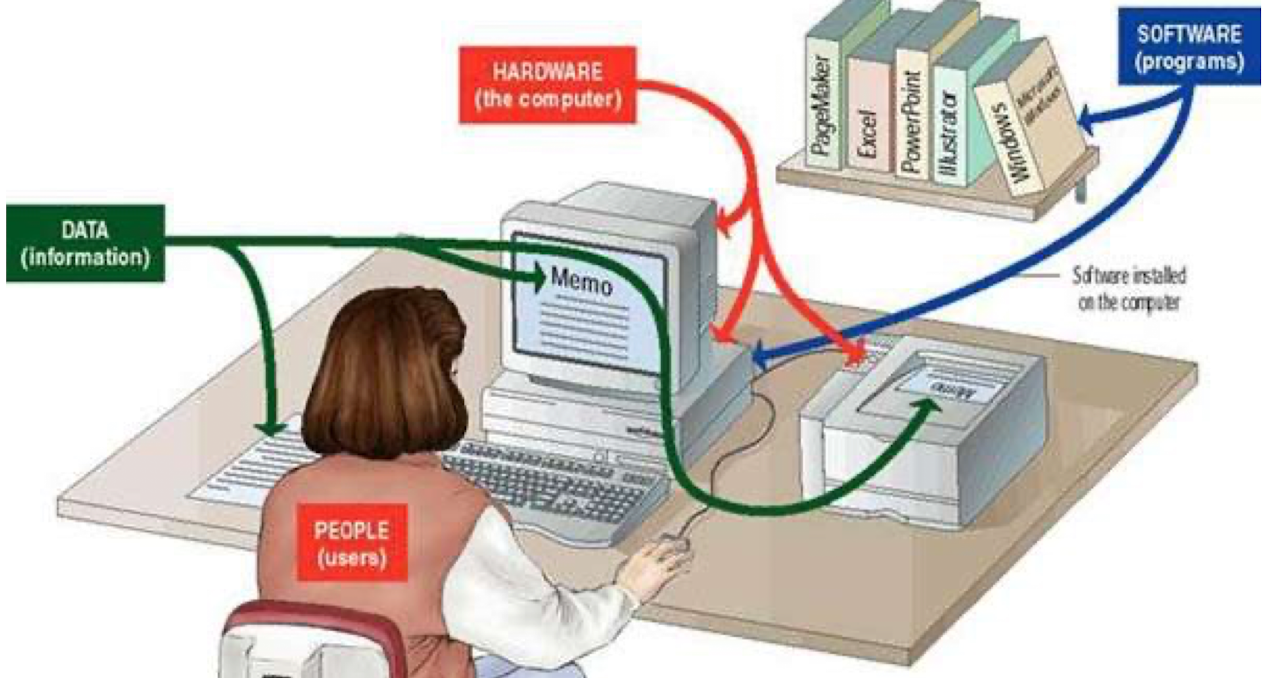
\includegraphics[width=7cm]{computer-system.png}\end{figure}
  \itm 컴퓨터 하드웨어의 블록 다이어그램: CPU는 메모리를 통해서만 데이터를 받을 수 있다. 입출력을 받는 메모리의 세 부분이 버퍼. 장치에서 온 데이터를 임시 저장하는 공간. 입력장치에서 출력을 내려면 메모리의 아웃풋 버퍼에 데이터를 전달해야 함. \begin{figure}[h]\centering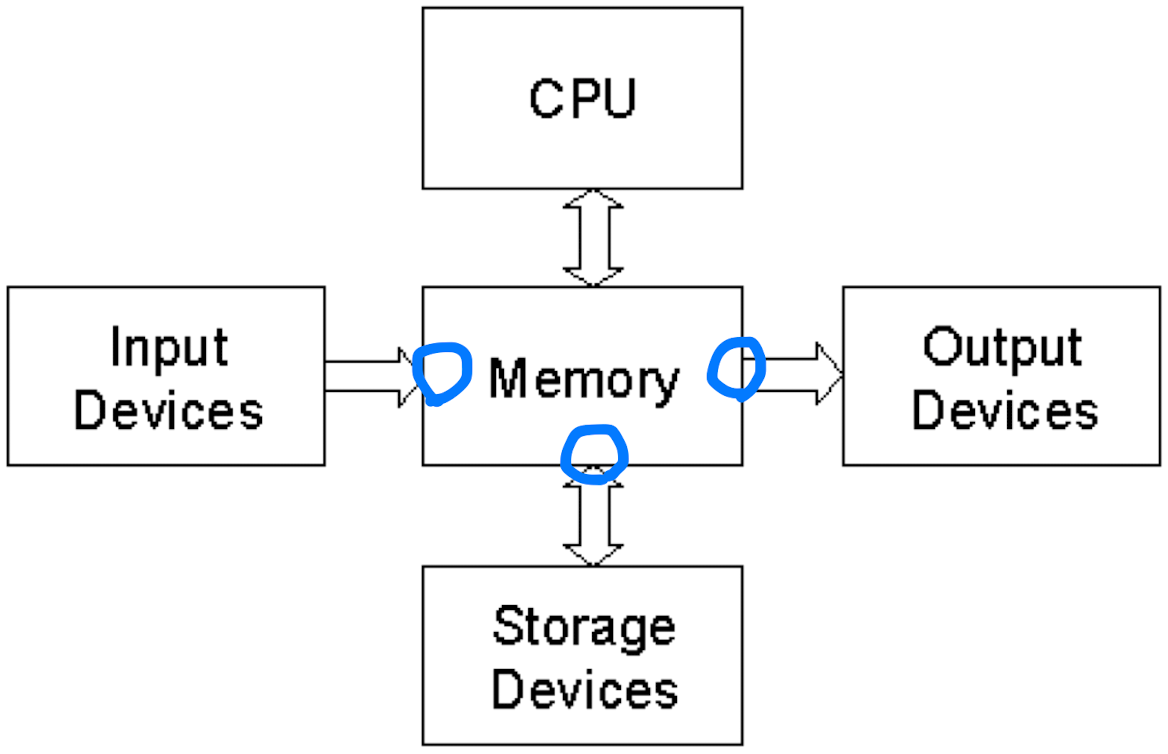
\includegraphics[width=7cm]{hardware-system.png}\end{figure}
  \itm 프로세스의 3가지 상태:
  \bitmz
    \itm RUN(FG, BG): 명령을 백그라운드로 실행.
    \itm KILL: <Ctrl-c>
    \itm STOP: <Ctrl-z>
  \eitmz
  \itm EOF: <Ctrl-d>
  \itm 리눅스 파일 시스템은 트리 구조.
\eitmz

\section{Shell}

\bitmz
  \itm \code{!!} \rarr 직전 명령.
  \itm \code{\$?} \rarr 직전 명령의 리턴 값(exit status).
  \itm \code{\$!} \rarr 직전 프로세스의 아이디. e.g., \code{kill -9 \$!}
  \itm \code{!so} \rarr 가장 최근에 실행한 so로 시작하는 명령.
  \itm \code{a\%b} \rarr a에서 b를 제외한 문자열을 반환.
  \itm create a gzipped archive and write it to a file: \code{tar czf path/to/target.tar.gz path/to/file1 path/to/file2 ...}
  \itm Extract a (compressed) archive file into the current directory verbosely: \code{tar xvf path/to/source.tar[.gz|.bz2|.xz]}
  \itm \code{drwx------} 디렉토리를 실행할 수 있나? \rarr 디렉토리는 실행이 아니라 \code{cd}로 접근 가능하다는 것.
  \itm \code{-r--rwxrwx oss000 foss} \rarr oss000은 \code{r--} 권한만 가짐. foss 그룹이더라도!
  \itm chmod a-x lab0522 \rarr lab0522에 대한 all의 x 권한이 사라짐.
  \itm \code{ls aaa bbb ccc |\& wc -l} \rarr 3

  \itm Expansion
  \bitmz
    \itm \code{echo "A=\$A"} \rarr \code{A=100}
    \itm \code{echo 'A=\$A'} \rarr \code{A=\$A} (no expansion)
    \itm \code{echo "ab\$Ade"} \rarr \code{ab}, Ade는 없는 변수이므로 \code{echo "ab\$\{A\}de"} 이렇게 해야 한다.
    \itm \code{echo `which cc`} \rarr \code{which cc} 명령이 실행됨.
    \itm \code{add `add 100 200` 300} \rarr \code{600}
    \itm \code{\{n..m..k\}} k 간격으로 n부터 m까지 출력.
    \bitmz
      \itm \code{echo \{a,b,c\}.js} \rarr \code{a.js b.js c.js}
      \itm \code{echo \{0..5\}} \rarr \code{1 2 3 4 5}
      \itm \code{echo \{0..10..3\}} \rarr \code{0 3 6 9}
      \itm \code{echo \{a..z\}} \rarr a부터 z
    \eitmz
    \itm \code{\$\{ \}} variable expansion
    \bitmz
      \itm \code{echo \$\{STR:(-3):3\}} \rarr STR의 마지막 세 번째 글자부터 세 글자.
      \itm \code{echo \$\{STR/from/to\}} \rarr STR의 from 문자열을 to로 변경.
      \itm \code{echo \$\{STR:-ALT\}} \rarr STR이 unset되어 있는 경우 ALT를 출력.
      \itm \code{echo \$\{STR:+ALT\}} \rarr STR이 set되어 있는 경우 ALT를 출력.
      \itm \code{echo \$\{PATH\#\#*.\}} \rarr PATH에서 .을 만날 때까지 문자를 제거. (extension)
      \itm \code{echo \$\{PATH\#\#*/\}} \rarr PATH에서 /를 만날 때까지 문자를 제거. (basename)
    \eitmz
    \itm \code{\$(( ))} numerical expansion: \code{echo $(( 100 + 200 ))$} \rarr 300
    \itm \code{\$( )} command substitution. 명령의 출력으로 치환한다. 백틱과 동일. e.g., \code{rm \$(cat file)}
  \eitmz

  \itm Loop
  \bitmz
    \itm \code{for i in /etc/*; do echo \$i; done} \rarr \code{/etc} 아래 모든 파일명을 출력.
    \itm \code{for ((i = 0 ; i < 100 ; i++)); do echo \$i; done}
    \itm \code{cat file | while read i; do echo \$i; done}
    \itm \code{sum=0; for i in \{1..10\}; do sum=\$(( \$sum+\$i )); echo \$i ":" \$sum; done}
    \itm \code{for i in \{000..999\}; do touch file\_\$\{i\}.c; done} \rarr file\_000.c부터 file\_999.c 파일 생성. 사실 touch는 파일 생성이 아니라 수정날짜를 바꾸는 명령.
    \itm \code{for i in file\_*; do mv \$i \$\{i\%.c\}.rs; done} \rarr file\_로 시작하는 파일들을 순회하며 문자열 끝의 .c를 .rs로 바꾼다.
    \itm \code{sum=0; for i in \{7..999..7\}; do sum=\$(( \$sum+\$i )); done; echo \$sum} \rarr 999까지의 모든 7의 배수 출력.
  \eitmz

  \itm Condition
  \bitmz
    \itm \code{if [[ condition ]]; then command1; elif [[ condition2 ]]; then command2; else command3; fi}
    \itm \code{if [[ -z \$STR ]]; then echo "empty"; else echo "not empty"; fi}
    \itm \code{if [[ \$STR1 == \$STR2 ]]; then echo "eq"; else echo "neq"; fi}
    \itm \code{if (( \$NUM1 < \$NUM2 )); then echo "lt"; else echo "gt"; fi} (bracket을 쓰면 숫자가 아니라 문자 순서 비교.)
    \itm \code{if command1; then command2; else command3; fi} \rarr command1의 exit status에 따른 분기.
  \eitmz
\eitmz

\section{Linux}

\bitmz
  \itm \code{ls} 파일 리스트.
  \bitmz
    \itm \code{ls file} \rarr 해당 파일이 있는지 여부. 있다면 stdout에 파일명을 출력, 없다면 stderr에 에러 메시지.
    \itm \code{ls -d dir} \rarr 디렉토리 내 파일 리스트가 아니라 dir을 출력. (해당 디렉토리가 있는지 여부) \code{ls -d}하면 . 출력.
    \itm \code{ls *.txt} \rarr \code{.txt}로 끝나는 모든 파일 출력.
    \itm \code{ls -i} \rarr INode를 함께 출력.
  \eitmz
  \itm \code{chmod [ugoa][+-][rwx] files...} 파일의 권한을 변경한다.
  \bitmz
    \itm rwx(user)rwx(group)rwx(others) = all
    \itm r(4), w(2), x(1): e.g., \code{chmod 700 file}
    \itm \code{-R} 디렉토리 내 모든 파일에 재귀적으로 적용.
    \itm default permission은 \code{-rw-r--r--}. 이것을 umask라고 한다.
    \itm 퍼미션 오른쪽 숫자는 같은 INode를 공유하는 링크 개수. 디렉토리의 경우에는 포함된 파일 개수.
  \eitmz

  \itm \code{mv} 파일이나 디렉토리를 이동한다.
  \bitmz
    \itm \code{\$ mv dir1 dir2} \rarr dir1을 통째로 dir2 아래로 옮긴다.
  \eitmz
\eitmz

\section{Git}

\begin{figure}[h]
  \centering
  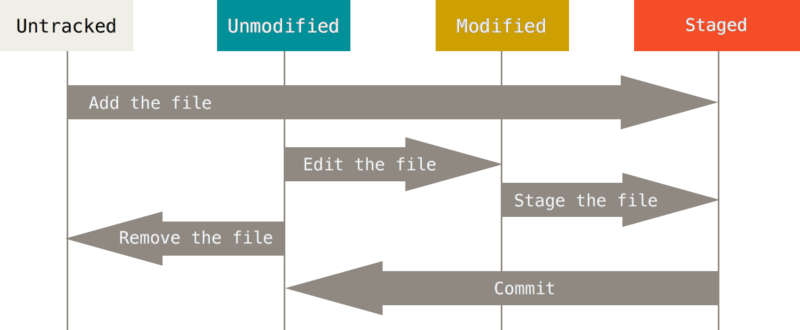
\includegraphics[width=5.2cm]{git-lifecycle.png}
  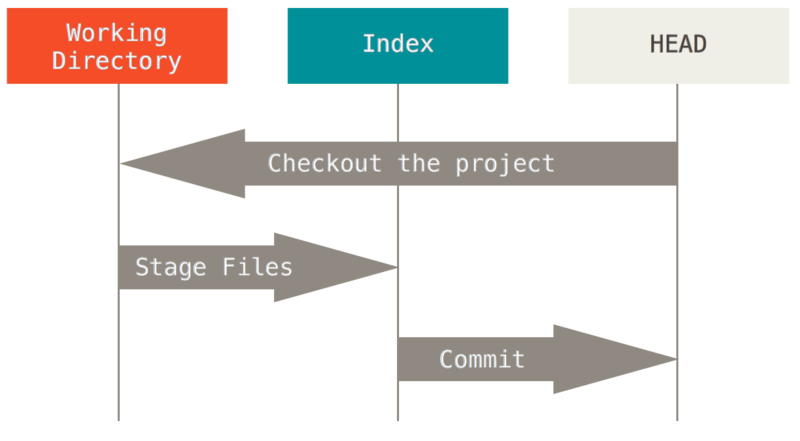
\includegraphics[width=4.3cm]{git-workflow.png}
\end{figure}

\bitmz
  \itm git: 소스코드 관리를 위한 형상 관리 소프트웨어. 분산 버전 관리 제공.
  \itm pull request, merge request의 뜻.
  \itm branch: 해당 프로젝트 내에서 기능 추가, 버그 픽스 등 작업할 때.
  \itm fork: 원본 프로젝트에 영향을 주지 않고, 해당 프로젝트를 기반으로 새로운 프로젝트를 만들 때.
  \itm \code{git reset [file]} \rarr unstage a file.
  \itm \code{git commit -m "message"} \rarr commit the staged content.
  \itm \code{git checkout} \rarr switch branches or restore working tree files.
  \itm \code{git branch} \rarr list your branches.
  \itm \code{git branch <branch-name>} \rarr create new branch at the current commit.
  \itm \code{git reset --hard [commit]} \rarr clear staging area, rewrite working tree from specified commit.
  \itm \code{git stash} \rarr save modified and staged changes.
\eitmz

\section{License}

\begin{figure}[h] \centering 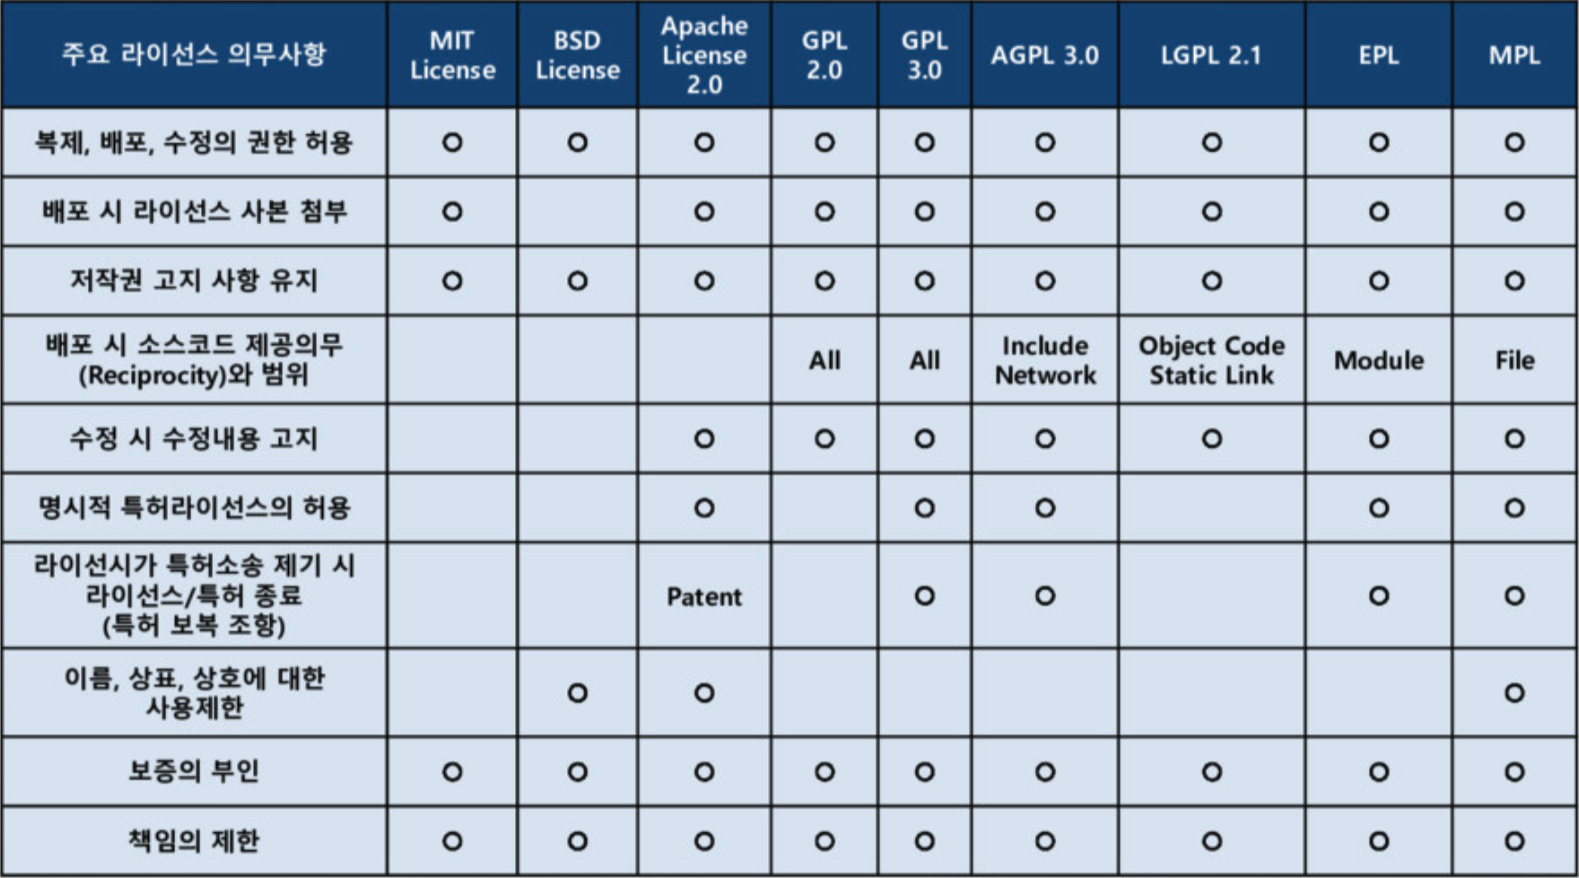
\includegraphics[width=\columnwidth]{oss-license.png} \end{figure}

\bitmz
  \itm 라이선스는 저작권자가 자신의 권리 일부를 일정 조건으로 사용할 권한을 허가, 부여하는 것. 저작권은 여전히 원 저작자에게 있고, 일부 사용에 대한 권리만 부여하는 것.
  \itm 오픈소스의 세가지 권리: 배포권, 사용권, 수정권. 이 셋을 보장하지 않는다면 오픈소스가 아님. 가령 MIT 라이센스에는 상업적 사용권이 있음. 여기에서 배포권 제한 불가.

  \itm 지식재산권에는 산업재산권, 저작권, 신지식재산권이 있음.
  \bitmz
    \itm 산업재산권:
    \bitmz
      \itm 특허: 원천/핵심기술, 자연법칙을 이용한 발명, 신규성, 진보성, 난이도, 산업 이용 가능성, 출원으로부터 20년.
      \itm 실용신안: 실용 개량기술, 고안, 고도하지 않아도 됨, 물품에 대해서만 인정, 출원으로부터 10년.
      \itm 디자인권: 물품의 디자인, 공업상 이용 가능성, 신규성, 창작성, 등록 시 발생, 등록/유사 디자인 권리 독점, 출원으로부터 20년.
      \itm 상표권: 상품 식별을 위한 표장, 기호, 자타상품식별력 필요, 등록 시 발생, 실시 권리 독점, 등록일로부터 10년, 10년 단위 갱신 가능. 도시명, 국가명은 상표 등록 불가. 타인이 유사 동일 상표 사용 불가.
    \eitmz
    \itm 저작권: 보호대상은 주관적인 창작이 인정되는 저작물. 저작자 자신의 독자적인 사상, 감정 표현을 담은 창작성을 갖춰야. 창작 시 권리 발생, 별도 등록 필요없음, (c) 선언, 저작자 사후 70년까지. 저작권자가 저작권을 갖는 것은 불변(MIT 라이센스라 할지라도). 법률, 행정문서에는 저작권 없음.
    \itm 신지식재산권: 산업저작권(소프트웨어), 첨단산업재산권(반도체, 영업방법, 생명공학기술), 정보재산권(DB, 영업비밀), 그 외 캐릭터, 프랜차이징, 퍼블리시티권 등.
  \eitmz

  \itm COPYLEFT: 저작권을 포기. 저작권을 다른 사람에게 부여. 저작물을 연구하고 사용할 자유, 다른 사람들과 같이 쓰고 복사할 자유, 수정할 자유, 2차 저작물을 배포할 자유. 단, 2차 저작물도 COPYLEFT를 따라야.

  \itm Creative Commons: 일정 규칙 하에 권리를 허용:
  \bitmz
    \itm CC BY: 저작자 표기 필요.
    \itm CC BY-SA: 라이센스 변경 불가.
    \itm CC BY-ND: 수정 불가.
    \itm CC BY-NC: 상업적 이용 불가.
  \eitmz

  \itm Free Software: 리처드 스톨만. 목적 불문 실행할 자유 + 프로그램 원리를 연구하고 변경할 자유(소스코드 제공 필요, 수정권) + 비상업적 목적으로 복제, 배포할 자유 + 수정한 버전을 배포할 자유. 상업성 반대, 전염.
  \itm Open Source Software: 에릭 레이몬드. 상업성 공존 인정. 자유 배포, 소스코드 포함, 2차 저작 허용, 다른 라이선스 수용, 라이선스의 기술적 중립성.

  \itm 오픈소스 라이선스: 무조건 배포, 사용, 수정권을 모두 허여해야.

  \bitmz
    \itm BSD/MIT: 수정된 소스코드를 공개하지 않아도 됨. 상업적 이용도 가능.
    \itm Apache2.0: 아파치라는 상표권을 침해해서는 안 됨. 수정한 코드를 공개하지 않아도 됨.
    \itm GPL2.0: 수정하거나 링크한 코드도 GPL 라이선스를 따라야. (네트워크 통신을 거쳐 사용하는 경우에는 전염되지 않음.) 배포 시 코드를 포함하거나 제공받을 방법을 명시해야. 특허가 포함된 경우 특허료를 포기해야.
    \itm GPL3.0: DRM 관련 이익을 포기해야. 특허를 개선해 배포한 경우 무료라는 라이센스 제공 필수, 특허 소송을 제기한 경우 제재가 가해짐.
    \itm LGPL2.1: 오픈소스를 장려하기 위한 전략적 라이선스. 링크한 경우에는 비공개 가능. 수정한 경우에는 코드 공개 필요. 하지만 특허는 GPL과 동일.
  \eitmz

  \itm 명시적 특허 라이선스 허용: 특허권이 있더라도 사용을 허용. 단, 특허권이 무효가 되는 것이 아님. 특허 사용을 허락한 것이 아니라, 그 특허가 포함된 소스코드의 사용을 허락한 것.
  \itm 책임의 제한, 보증의 부인: 오픈소스 저작자는 책임과 보증을 부인할 권리가 있음. 오픈소스 코드가 포함된 제품에 문제가 생기는 경우 해당 오픈소스 저작자가 책임, 보증할 필요 없음.
\eitmz

\section{Biz}

\bitmz
  \itm 오픈소스 코드를 수정해서 수익을 내면 라이센스 위반일 수 있지만, 교육, 훈련, 기술지원, 자문 등으로 수익 추구를 할 수 있음. 브랜드, SaaS, 기부, 크라우드소싱도 가능.
  \itm 펀딩 단체와 제휴, 광고 수익, 듀얼 라이선스(e.g., 특허 부분은 오픈소스로 공개하지 않음), 인증 제공, 특정 버전까지만 무료, 난독화, 추가 기능 유료 정책 가능.
  \itm 오픈소스 소프트웨어를 구동하기 위한 하드웨어를 판매할 수도, GPLv3는 불가능.
\eitmz
